\documentclass[11pt]{article}
\usepackage[utf8]{inputenc}
\usepackage{graphicx}
\usepackage{amsmath}
\usepackage{amsfonts}
\usepackage{hyperref}
\usepackage{listings}
\usepackage{courier}
\usepackage[letterpaper, portrait, margin=1in]{geometry}
\graphicspath{/home/black/CPS/euler}

\lstset{
	basicstyle=\footnotesize\ttfamily,
	frame=single,
	breaklines=true
}

\title{\vspace{-1.5cm}Project Eueler 107}
\author{Kevin Black}

\begin{document}

\maketitle

\section{Problem Statement}

A k-input binary truth table is a map from k input bits (binary digits, 0 [false] or 1 [true]) to 1 output bit.

How many 6-input binary truth tables, $\tau$, satisfy the formula

\begin{center}
	$\tau(a, b, c, d, e, f)$ AND $\tau(b, c, d, e, f, a$ XOR $(b$ AND $c)) = 0$
\end{center}

for all 6-bit inputs $(a, b, c, d, e, f)$? 

\section{Code}
\lstinputlisting[language=Python]{209.py}

\section{Rationale}
First, I decided to examine the transformation $(a, b, c, d, e, f) \to (b, c, d, e, f, a$ XOR $(b$ AND $c))$. The line \verb!inputs = list(product([False, True], repeat=6))! creates a list of all possible combinations of 6 binary values (all 64 inputs to the truth table). I then used the graphviz library to examine the nature of this transformation (defined by the method \verb!transform!) on these 64 inputs. The result was the following:

\begin{center}
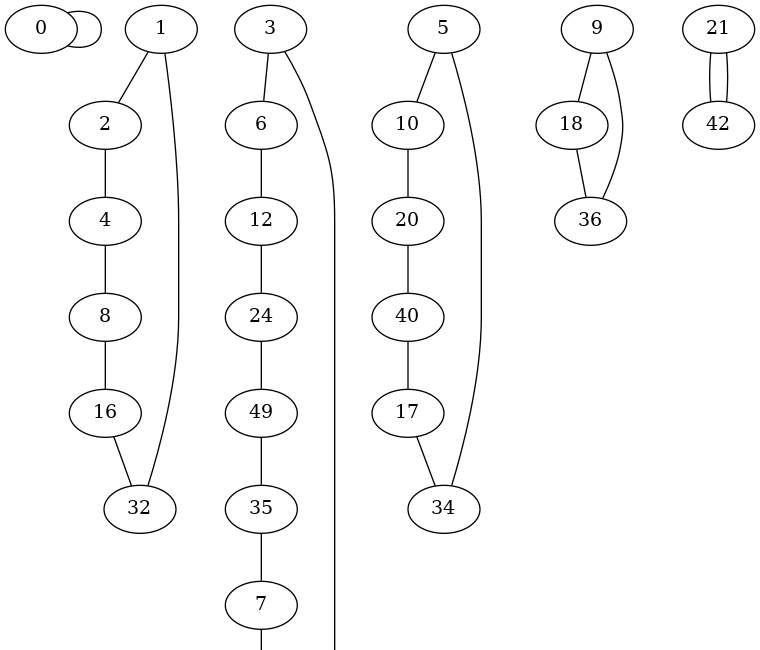
\includegraphics[scale=0.5]{/home/black/CPS/euler/graph.png}
\end{center}

By observing this visualization, it is clear that the input transformation forms 6 disjoint cycle graphs of lengths 1, 2, 3, 6, 6, and 46 (the one of length 46 is cut off in the picture; it continues downward quite a ways).

Each edge in the graph represents a connection between an input $(a, b, c, d, e, f)$ and $(b, c, d, e, f, a$ XOR $(b$ AND $c))$. In order for $(a, b, c, d, e, f)$ AND $(b, c, d, e, f, a$ XOR $(b$ AND $c))$ to be 0 for all inputs, no two adjacent nodes in the graph can be 1. The number of ways for this to happen is just the number of ways for this to happen for each cycle multiplied together.

I derived the number of ways to assign 0s and 1s to an $n$-cycle such that no two adjacent nodes are 1 to be the following:

\begin{align*}
	\sum_{k=0}^{n} \binom{n - k + 1}{k} - \binom{n - k - 1}{k - 2}
\end{align*}

I will explain the derivation on the board. An interesting note is that this expression turns out to just be the $nth$ Lucas number (the Fibonacci sequence with starting values of 2 and 1).

The method \verb!combs! implements this expression naively using the binomial coefficient. The final bit of code finds all the cycles in the transformation, counting their lengths, and then multiplies together the number of possibilites for each cycle to find the answer. 


\end{document}